\documentclass[sigconf,nonacm]{acmart}

\setcopyright{none}
\settopmatter{printacmref=false}
\renewcommand\footnotetextcopyrightpermission[1]{}
\pagestyle{plain}
\setlength{\headheight}{15.2pt}

\usepackage{graphicx}
\usepackage{booktabs}
\usepackage{array}
\usepackage{amsmath}
\usepackage{tabularx}

\newcolumntype{Y}{>{\raggedright\arraybackslash}X}

\title[Experiment Report on Text-to-3D Generation with MTN]{Experiment Report on Text-to-3D Generation with MTN: A Tiger Doctor Case Study}

\author{Student Name}
\affiliation{%
  \institution{University of Macau}
  \city{Macau}
  \country{China}
}
\email{student@um.edu.mo}

\begin{document}

\begin{abstract}
This report studies text-to-3D generation with MTN under a course-style experimental setting. The target prompt is \textit{a tiger dressed as a doctor}, and the goal is to obtain at least one usable 3D result, monitor GPU memory behavior, analyze failures, and examine hyper-parameter sensitivity. Six representative runs were organized around DeepFloyd-IF guidance, resolution control, learning-rate adjustment, and perpendicular negative prompting. The best result was produced by a DSLR-style prompt without \texttt{perpneg} at $64\times 64$, while the most severe failures were early out-of-memory termination and geometry collapse into a glowing sphere. The experiments show that prompt formulation and guidance configuration matter more than simply increasing constraint strength, and that memory-aware configuration is necessary before visual quality can even be discussed.
\end{abstract}

\maketitle

\section{Introduction}
Recent text-to-3D systems optimize a radiance field or related 3D representation by matching rendered views against large diffusion priors \cite{poole2022dreamfusion, yi2026progressive}. MTN is a practical implementation of this idea, and its repository exposes a number of user-facing controls such as diffusion backbone, image resolution, learning rate, and negative-guidance settings \cite{texaser-mtn-repo}. In practice, these controls are tightly coupled: a setting that improves one prompt may destabilize another, and an apparently minor change can shift the bottleneck from semantic alignment to GPU memory.

This report focuses on a single prompt family, \textit{tiger doctor}, because it is semantically rich enough to expose both appearance and geometry failures. The report has three goals. First, it documents the final successful result and the commands that produced it. Second, it treats failures as first-class outcomes rather than discarded runs. Third, it summarizes which hyper-parameters were helpful, harmful, or simply too expensive for the available hardware budget.

\section{Experimental Setup}
All experiments were conducted in the MTN codebase \cite{texaser-mtn-repo} using the IF guidance path. The recorded environment in the lab notes was Python 3.9, CUDA 12.8, and PyTorch 2.8.0. GPU usage was monitored with \texttt{gpustat}, and the logs indicate an approximately 24.6 GB GPU budget. Each run used 6000 iterations with batch size 1. Qualitative evaluation followed the course requirement: the resulting 360$^{\circ}$ videos were inspected for geometry integrity, texture quality, and multi-view consistency.

The experiments covered three groups:
\begin{itemize}
    \item Low-memory baselines at $48\times 48$ for stable comparison.
    \item Resource-stress runs with \texttt{perpneg} to expose memory and optimization failures.
    \item DSLR-style prompt refinement to test whether better prompt phrasing outperforms stronger negative guidance.
\end{itemize}

\section{Main Results}
Table~\ref{tab:results} summarizes the most relevant runs. The low-memory IF baseline was stable but blurry. Increasing the learning rate from $1\times 10^{-3}$ to $3\times 10^{-4}$ under the project's effective scheduler setting slightly improved sharpness, but did not solve semantic drift or shape artifacts. The most important observation came from the DSLR prompt experiments: removing \texttt{perpneg} produced the only clearly presentable result, while keeping strong negative guidance caused geometry collapse even when the run completed.

\begin{table*}[t]
\caption{Summary of representative MTN runs for the tiger-doctor prompt family. Geometry, texture, and consistency are subjective scores on a 1--4 scale derived from the experiment log.}
\label{tab:results}
\centering
\footnotesize
\setlength{\tabcolsep}{4pt}
\renewcommand{\arraystretch}{1.15}
\begin{tabularx}{\textwidth}{p{2.3cm} p{2.7cm} c c c c c Y}
\toprule
Workspace / name & Key setting & Time & Peak VRAM & Geo. & Tex. & Cons. & Observation \\
\midrule
\shortstack[l]{trial\_if\\lowmem} & IF, \texttt{vram\_O}, $48\times48$ & 17.77 min & 12.0 GB & 2 & 1 & 2 & Stable but blurry; the object remains barely recognizable. \\
\shortstack[l]{trial\_if\\lr3e4} & IF, \texttt{vram\_O}, $48\times48$, \texttt{lr=3e-4} & 17.44 min & 12.0 GB & 2 & 2 & 2 & Slightly clearer than the baseline, but still affected by semantic drift and strong artifacts. \\
\shortstack[l]{trial\_if\\perpneg} & IF, \texttt{perpneg}, default $64\times64$ & early fail & OOM & -- & -- & -- & Training terminates before any usable output is produced. \\
\shortstack[l]{trial\_if\\perpneg\\lowmem} & IF, \texttt{perpneg}, \texttt{vram\_O}, $48\times48$ & 103.98 min & 13.8 GB & 1 & 1 & 1 & The run is slow and converges to volumetric noise rather than a coherent subject. \\
\shortstack[l]{trial\_perpneg\\if\_tiger\\baseline\_6000} & DSLR prompt, \texttt{perpneg}, \texttt{negative\_w=-3.0}, $48\times48$ & 69.62 min & 13.8 GB & 1 & 1 & 1 & The geometry collapses into a bright sphere and the tiger-doctor semantics disappear. \\
\shortstack[l]{trial\_if\_tiger\\no\_perpneg\_64} & DSLR prompt, no \texttt{perpneg}, \texttt{vram\_O}, $64\times64$ & 21.78 min & 17.6 GB & 4 & 4 & 4 & Best overall result with recognizable appearance and consistent multi-view structure. \\
\bottomrule
\end{tabularx}
\end{table*}

\begin{figure*}[t]
    \centering
    
\includegraphics[width=0.24\linewidth]{../exp3/screenshots/trial-if-tiger-no-perpneg-64-1.png}\hfill
    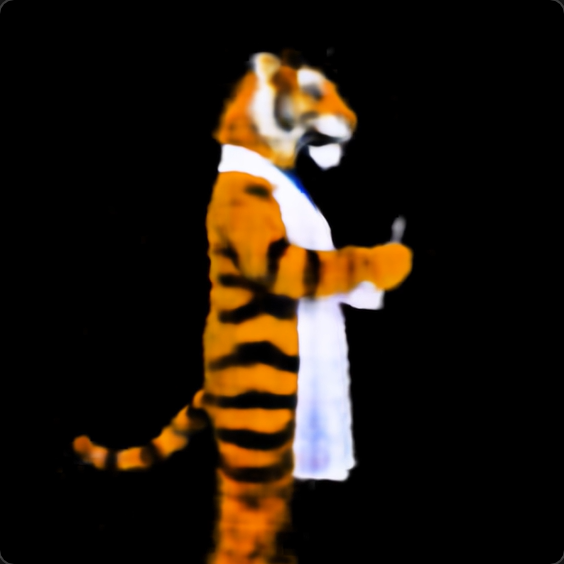
\includegraphics[width=0.24\linewidth]{../exp3/screenshots/trial-if-tiger-no-perpneg-64-2.png}\hfill
    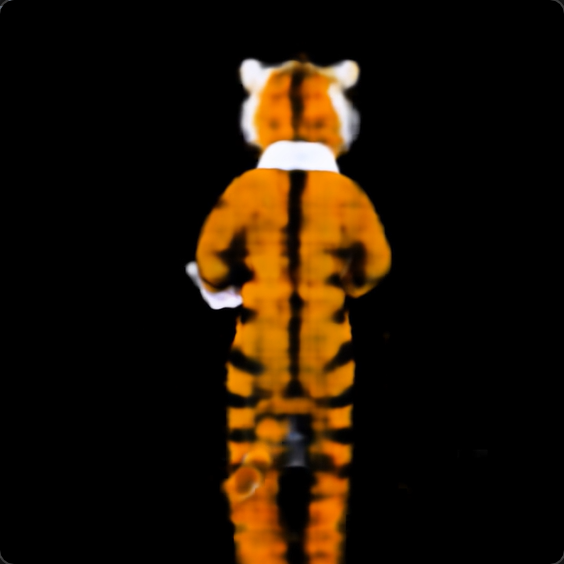
\includegraphics[width=0.24\linewidth]{../exp3/screenshots/trial-if-tiger-no-perpneg-64-3.png}\hfill
    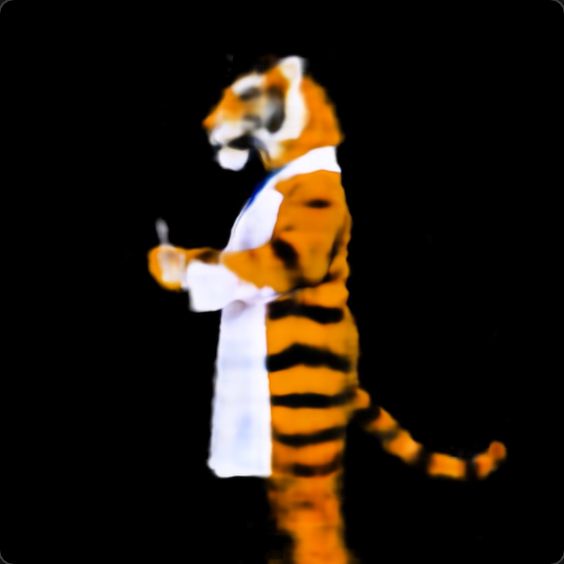
\includegraphics[width=0.24\linewidth]{../exp3/screenshots/trial-if-tiger-no-perpneg-64-4.png}
    \Description{Four screenshots of the best MTN result showing a tiger dressed as a doctor from multiple viewpoints. The figure demonstrates a coherent orange tiger body, a white coat, and stable side and rear views.}
    \caption{Best result from \texttt{trial\_if\_tiger\_no\_perpneg\_64}. The model produces a recognizable tiger doctor with a readable lab coat silhouette and substantially better multi-view consistency than the other runs.}
    \label{fig:best-result}
\end{figure*}

The successful run in Figure~\ref{fig:best-result} is still imperfect. The lab coat is somewhat over-smoothed, the face remains slightly blurry, and Janus-like ambiguity is still visible around the head. However, compared with all baseline and failure cases, this run is the only one that consistently preserves identity, clothing semantics, and body shape across viewpoints.

\section{Failure Analysis}
Two failures were especially informative because they represent different failure types.

\subsection{F1: OOM as a Resource Failure}
The default IF + \texttt{perpneg} run at $64\times64$ terminated before the first valid render was produced, so the evidence for this case comes from runtime logs rather than output images. This makes it a resource failure rather than a visual failure.

\begin{table}[t]
\caption{Runtime evidence for the F1 OOM case.}
\label{tab:f1-oom}
\centering
\footnotesize
\setlength{\tabcolsep}{4pt}
\renewcommand{\arraystretch}{1.12}
\begin{tabular}{p{0.22\linewidth} p{0.70\linewidth}}
\toprule
Item & Evidence \\
\midrule
Command & \texttt{main.py -O --workspace trial\_if\_perpneg --IF --perpneg} with the tiger-doctor prompt and 6000 iterations. \\
Symptom & Training aborts before the first evaluation with \texttt{torch.OutOfMemoryError: CUDA out of memory}. \\
Memory evidence & A closely related $64\times64$ IF + \texttt{perpneg} run with \texttt{--vram\_O} already reaches \texttt{20.5GB} GPU usage in the log excerpt, leaving little headroom for the non-optimized setting. \\
Implication & The configuration exceeds the practical memory budget on the available GPU and should be treated as an infeasible setup. \\
\bottomrule
\end{tabular}
\end{table}

The log evidence is sufficient to explain the failure mechanism: the combination of IF guidance, default resolution, and perpendicular negative prompting creates a memory load that is too high for the current hardware budget.

\subsection{F2: Geometry Collapse under Strong Negative Guidance}
Unlike F1, the DSLR prompt with \texttt{perpneg} and \texttt{negative\_w=-3.0} finished training, so it produced a proper visual failure case. Figure~\ref{fig:f2-collapse} shows that the output collapses into a bright orange sphere-like volume instead of a tiger doctor. This indicates that the system remained numerically stable while converging to an unusable geometry.

\begin{figure}[t]
    \centering
    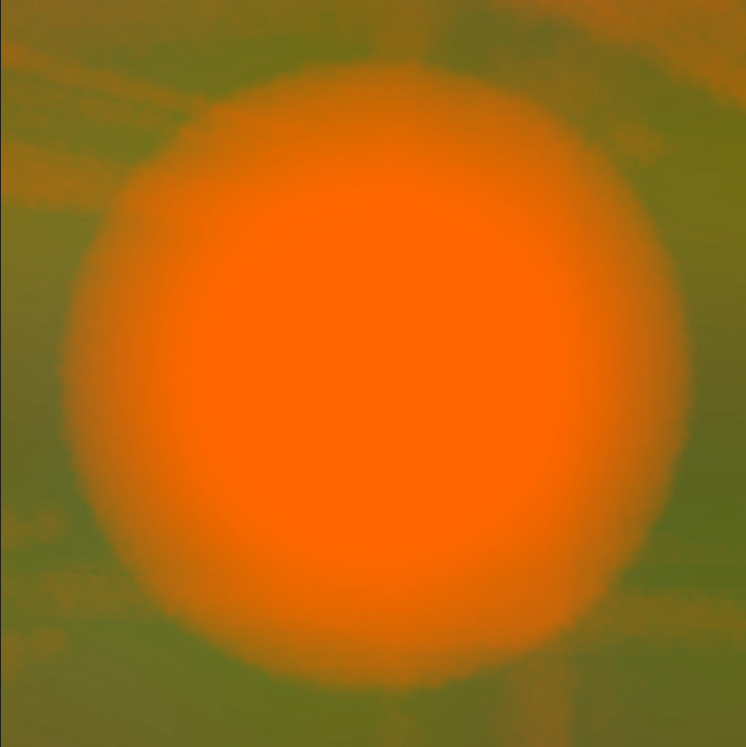
\includegraphics[width=0.48\linewidth]{../exp3/screenshots/f2-dslr-tiger-perpneg-1.png}\hfill
    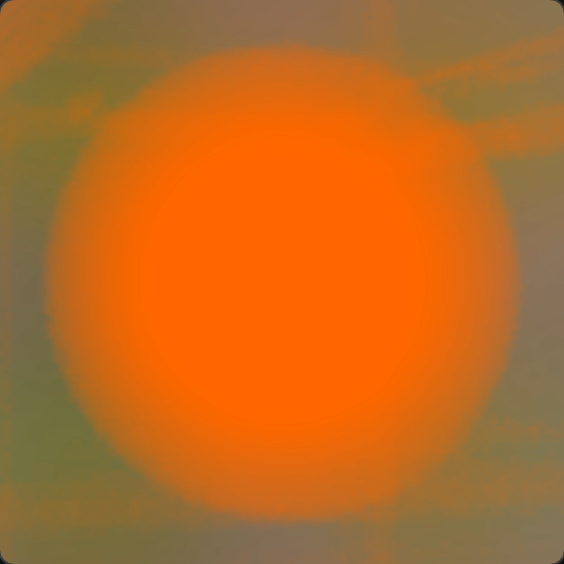
\includegraphics[width=0.48\linewidth]{../exp3/screenshots/f2-dslr-tiger-perpneg-2.png}
    \Description{Two screenshots of the failure case under strong perpendicular negative guidance. Both views show a bright orange spherical object without recognizable tiger or doctor structure.}
    \caption{F2 failure case under strong perpendicular negative guidance. The model no longer represents a tiger doctor and instead collapses into a glowing volumetric sphere.}
    \label{fig:f2-collapse}
\end{figure}

The contrast between F2 and \texttt{trial\_if\_tiger\_no\_perpneg\_64} suggests that the prompt itself was not the core problem. The decisive factor was the guidance strategy. For this prompt, adding strong perpendicular negative guidance over-constrained the optimization and suppressed stable object formation.

\section{Hyper-Parameter Reflection}
The experiments reveal three practical lessons.

First, memory-aware configuration is a prerequisite rather than a final optimization. Lowering the render resolution from $64\times64$ to $48\times48$ and enabling \texttt{vram\_O} successfully avoided OOM in several runs, but this alone did not guarantee visual quality. In fact, the low-memory \texttt{perpneg} run took 103.98 minutes and still produced unusable 3D noise.

Second, learning-rate adjustment had limited but real effect. The \texttt{lr=3e-4} baseline was slightly sharper than the default low-memory baseline, but the gain was incremental rather than transformative. This indicates that for this task, optimization hyper-parameters are secondary to prompt formulation and guidance design.

Third, removing a harmful constraint can be more effective than adding stronger control. The strongest positive result came from deleting \texttt{perpneg} in \texttt{trial\_if\_tiger\_no\_perpneg\_64}. This change improved semantics, geometry, and consistency simultaneously, while also reducing runtime relative to the DSLR + \texttt{perpneg} comparison.

\section{Improvement Suggestions}
Based on the above observations, two concrete improvements are recommended.

\noindent\textbf{1) Use staged resolution and guidance schedules.} A practical strategy is to begin at $48\times48$ without \texttt{perpneg} to secure a stable coarse shape, and only then test higher resolution or mild negative guidance. This should reduce wasted long runs that fail early or collapse late.

\noindent\textbf{2) Replace strong negative guidance with prompt refinement and seed control.} The DSLR-style prompt clearly helped semantic formation more than aggressive \texttt{negative\_w}. Future runs should prioritize prompt wording, fixed seeds, and milder regularization before attempting strong negative-view constraints.

An additional engineering recommendation is to add an early memory screening stage. A short pilot run of several epochs can reveal whether a configuration is already near the hardware limit, which would have flagged the OOM-prone settings sooner.

\section{Conclusion}
This experiment achieved the core lab goals: one presentable text-to-3D result was produced, GPU memory was monitored, at least two failures were analyzed, and hyper-parameter sensitivity was examined. The main conclusion is that for MTN under IF guidance, memory optimization is necessary but not sufficient. The decisive gain came from choosing a prompt and guidance combination that preserved semantic structure instead of over-constraining it. For the tiger-doctor prompt family, the no-perpneg DSLR run delivered the strongest overall result, while the most informative failures were early OOM and guidance-induced geometry collapse.

\bibliographystyle{ACM-Reference-Format}
\bibliography{mtn_refs}

\end{document}